\documentclass[pdf]{beamer}

\usepackage[croatian]{babel}
\usepackage[utf8x]{inputenc}

\PreloadUnicodePage{2}
\PrerenderUnicode{č}
\PrerenderUnicode{ć}
\PrerenderUnicode{ž}

%\usetheme{Montpellier}

\mode<presentation>{}

\subject{Diplomski rad br. 1115}

\title{Duboke konvolucijske neuronske mreže za raspoznavanje znakova}

%\subtitle{Diplomski rad br. 1115}

\author{Matija Ilijaš}

\begin{document}

%% title frame
\begin{frame}
\titlepage
\end{frame}

\section*{Sadržaj}
\begin{frame}
 \frametitle{Sadržaj}
 \tableofcontents[]%pausesections]
\end{frame}


\section{Optičko prepoznavanje znakova}

\begin{frame}{Optičko prepoznavanje znakova}

\begin{itemize}
\setlength\itemsep{0.5em}
	\item engl. Optical Character Recognition - OCR

	\item  Područje računalnog vida, raspoznavanja uzoraka 
	
 	\item  Dva glavna zadatka OCR sustava: 
	 \begin{itemize}
	 	\item Segmentacija znakova iz slike
	 	\item  Klasifikacija znakova
	\end{itemize}
	
 	\item U ovom radu analiziraju se metode klasifikacije
 	
 	\item Standarna metoda provodi se u dva koraka:
 	 \begin{itemize}
	 	\item Predprocesiranje slike znaka
	 	\item  Klasifikacija znaka
	\end{itemize}
 	
\end{itemize}

\end{frame}


\section{Umjetne neuronske mreže}

\begin{frame}{Umjetne neuronske mreže}

\begin{itemize}
\setlength\itemsep{0.5em}
	\item Algoritam strojnog učenja inspiriran strukturom i funkcionalnošću ljudskog mozga

 	\item  Paralelna obrada podataka, nelinearna veza ulaza i izlaza
	\item Neuron - težinska suma ulaza sa dodanom nelinearnošću
	 \item Standarna arhitektura neuronske mreže
 	\begin{itemize}
 		\item Potpuno povezana i aciklička
 		\item Sigmoidalna prijenosna funkcija
 	\end{itemize}
 
\end{itemize}

\begin{figure}
\centering
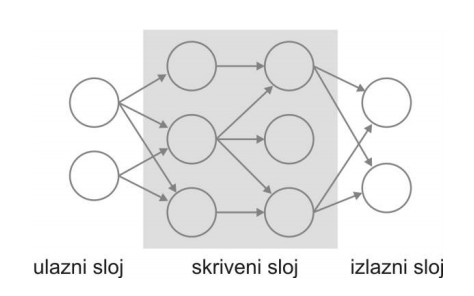
\includegraphics[width=6cm]{slike/neural_architecture.png}
\end{figure}

\end{frame}

\begin{frame}{Učenje neuronskih mreža}

\begin{itemize}
\setlength\itemsep{0.5em}

	\item Neuronska mreža - nelinearna funkcija sa više varijabli

 	\item Učenje mreže - traženje minimuma te funkcije s obzirom na grešku klasifikacije

	\item Koristi se Backpropagation algoritam koji implementira metodu gradijentnog spusta 
	
\end{itemize}

\begin{figure}
\centering
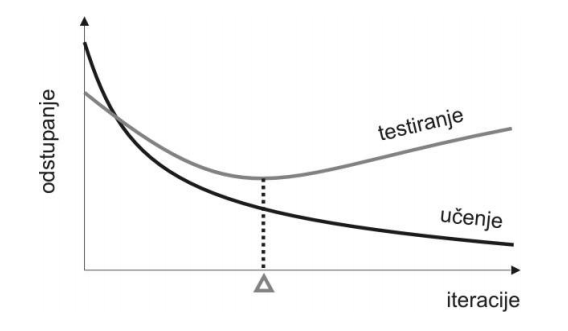
\includegraphics[width=7cm]{slike/generalization.png}
\end{figure}
 		
\end{frame}


\section{Duboko učenje}

\begin{frame}{Duboko učenje}

\begin{itemize}
\setlength\itemsep{0.5em}

	\item Ideja prvi put prezentirana u radovima Kunihika Fukushime i Yanna Lecuna prije gotovo 30 godina

 	\item Učenje korisnih značajki podataka povezanih u obliku hijerarhije - inspirirano vizualnim korteksom mozga sisavaca

	\item Uče se duboki kompleksni modeli na velikoj količini podataka - tek nedavno postalo moguće učenjem na grafičkim karticama 
	
	\item Metode nenadziranog učenja
	\begin{itemize}
		\item Učenje hijerarhije na neoznačenim podatcima
 		\item Autoenkoderi, ograničeni Boltzmann strojevi
 	\end{itemize}
 	
 	\item Metode nadziranog učenja
	\begin{itemize}
		\item Učenje Backpropagation algoritmom
 		\item Specijalne arhitekture (npr. konvolucijske)
 	\end{itemize}
	
\end{itemize}
. 
\end{frame}

\begin{frame}{Učenje hijerarhije značajki}

\begin{itemize}
\setlength\itemsep{0.5em}

	\item Kvalitetna značajka - diskriminantna, robusna na promjene osvijetljenja i geometrijske transformacije
	
	\item Ručno određivanje značajki - promatranje svojstva ulaznih podataka te naglašavanje onih maksimalno diskriminantnih
	
	\item Negativna posljedica ručnog određivanja je gubitak dijela korisnih informacija
	
	\item Rješenje: određivanje diskriminantnih značajki izravno iz skupa podataka

	\item Jedna razina apstrakcije - LDA i PCA metoda
	
	\item Više razina apstrakcije - hijerarhija značajki naučena dubokim učenjem na skupu podataka
		
\end{itemize}

\end{frame}

\begin{frame}{Učenje hijerarhije značajki}

\begin{figure}[ht!]
\centering
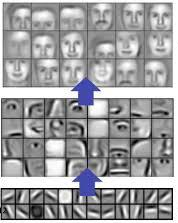
\includegraphics[height=7cm]{slike/feature_hierarchy.png}
\end{figure}

\end{frame}


\section{Duboke konvolucijske mreže}

\begin{frame}{Duboke konvolucijske mreže}

\begin{itemize}
\setlength\itemsep{0.5em}

	\item  Prvi model razvio Yann Lecun 1989. godine 
	
	\item Iskorištavaju svojstvo lokalne prostorne korelacije prirodnih slika
	
	\item Lokalni prostorni filteri ostvareni konvolucijom oponašaju lokalne receptore vizualnog korteksa


	\item Cilj je naučiti konvolucijske jezgre specifične za dane podatke - učenje lokalnih  značajki iz podataka

	\item Prvi dio arhitekture zadužen za formiranje hijerarhije značajki, drugi za klasifikaciju
	
	\item Nadzirano učenje Backpropagation algoritmom 
	
\end{itemize} 
 
\end{frame}

\begin{frame}{Lokalni prostorni filteri}

\begin{equation}
		y(m,n) = x(m,n)  \ast h(m,n) = \sum\limits_{j=-\infty}^{\infty} \sum\limits_{i=-\infty}^{\infty} x(i,j) h(m-i,n-j)  \nonumber
\end{equation}

\begin{figure}
\centering
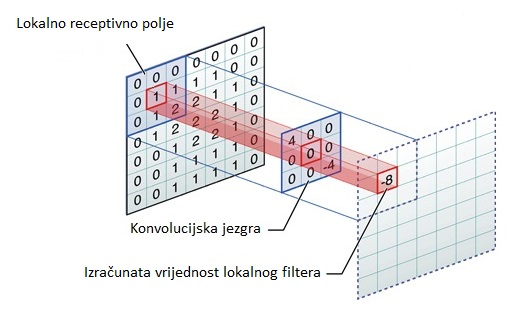
\includegraphics[width=10cm]{slike/kernel_convolution.jpg}
\end{figure}
	
\end{frame}

\begin{frame}{Dijeljenje težina}

\begin{itemize}
\setlength\itemsep{0.5em}

	\item  Naučeni lokalni filter prepoznaje lokalnu značajku na samo jednoj poziciji u prostoru 
	
	\item Mapa značajki - skup inačica lokalnih filtera koje pokrivaju sve moguće podprostore
	
	\item Element konvolucijskog sloja je matrica vrijednosti odziva  pripadajućeg filtera za svaku poziciju u prostoru

	\item Dijeljenjem težina između parametara mreže smanjuje se ukupan broj slobodnih parametara, te se kao posljedica:
	
	\begin{itemize}
		\item Smanjuje trajanje učenja
 		\item Poboljšava sposobnost generalizacije 
 	\end{itemize}

	
\end{itemize} 

\end{frame}

\begin{frame}{Dijeljenje težina}

\begin{figure}
\centering
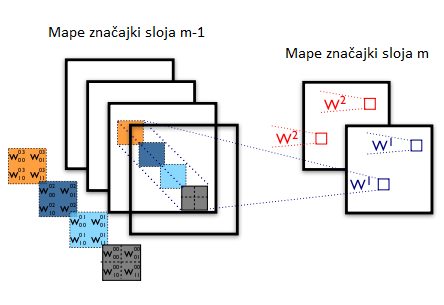
\includegraphics[width=10cm]{slike/shared_weights.png}
\end{figure}

\end{frame}

\begin{frame}{Lokalno udruživanje}

\begin{itemize}
\setlength\itemsep{0.5em}

	\item engl. Pooling
 
	\item  Oblik nelinearnog poduzorkovanja
	
	\item Slika se dijeli na nepreklapajuće podprozore fiksne veličine
	
	\item Maksimalno lokalno udruživanje -  uzimanje maksimalne vrijednosti svakog podprozora 
	
	\item Koriste se kao dodatni sloj nakon svakog sloja konvolucije, što
	
	\begin{itemize}
		\item smanjuje količinu računanja u višim slojevima
 		\item  ostvaruje jedan oblik invarijantnosti na translaciju 
 	\end{itemize}

	
\end{itemize} 

\end{frame}

\begin{frame}{Lokalno udruživanje}

\begin{figure}
\centering
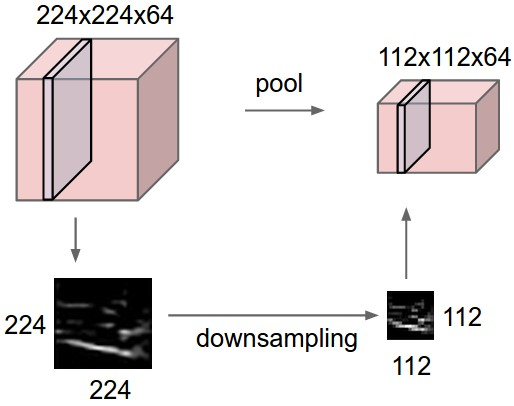
\includegraphics[width=9cm]{slike/max_pooling.jpeg}
\end{figure}

\end{frame}

\begin{frame}{Ispravljena linearna jedinica}

\begin{itemize}
\setlength\itemsep{0.5em}

	\item engl. Rectified Linear Unit - ReLU
 
	\item  Rješava problem nestajućeg gradijenta
	
	\item Ubrzava učenje svojim jednostavnim računanjem
\end{itemize} 

\begin{equation}
f(x) = \text{max}(x, 0) \nonumber     
\end{equation}

\begin{figure}
\centering
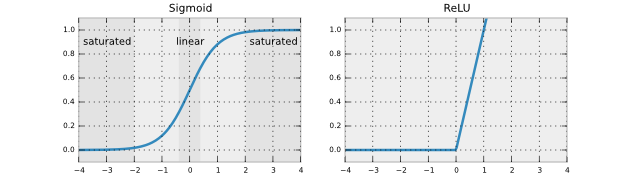
\includegraphics[width=10cm]{slike/sigmoid_relu.png}
\end{figure}

\end{frame}

\begin{frame}{Konačni model}

\begin{itemize}
\setlength\itemsep{0.5em}

	\item Sastoji se od slojeva za formiranje hijerarhije značajki i slojeva za klasifikaciju

	\item Svaki sloj za formiranje hijerarhije sastoji se od:
	\begin{itemize}
		\item  Konvolucijskog sloja 
		\item Sloja ispravljenih linearnih jedinica
 		\item  Sloja maksimalnog lokalnog udruživanja
 	\end{itemize}
 	
 	\item Slojevi za klasifikaciju su standarni i potpuno povezani
 
\end{itemize} 

\begin{figure}[ht!]
\centering
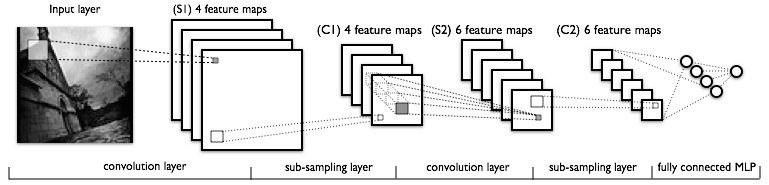
\includegraphics[width=11cm]{slike/convnet.jpg}
\end{figure}

\end{frame}

\section{Implementacija}

\begin{frame}{Implementacija}

\begin{itemize}
\setlength\itemsep{0.5em}

	\item Sustav za učenje i testiranje različitih arhitektura neuronskih mreža

	\item Prilikom razvijanja zadovoljena dva glavna uvjeta: 
	\begin{itemize}
 		\item Brzo učenje kompleksnih modela na velikoj količini podataka
 		\item Detaljna analiza rada naučenih modela
	\end{itemize}
	
	\item Sustav je podijeljen na dva podsustava razvijena sa zasebnim alatima:
	\begin{itemize}
 		\item Sustav za učenje
 		\item Sustav za testiranje
	\end{itemize}
	
	\item Dodatno implementirana prilagodba OCR sustavu tvrtke Microblink
	
\end{itemize}



\end{frame}


\begin{frame}{Sustav za učenje}

\begin{itemize}
\setlength\itemsep{0.5em}

	\item Implementiran u razvojnom alatu Torch koji omogućuje paralelno izvođenje procesa učenja na grafičkoj kartici
	
	\item Napisane skripte u jeziku LuaJIT za lagano definiranje arhitektura mreža i određivanje parametara učenja
	
	\item Naučeni Torch modeli se spremaju u posebnom formatu i šalju sustavu za testiranje
	
\end{itemize}

\begin{figure}
\centering
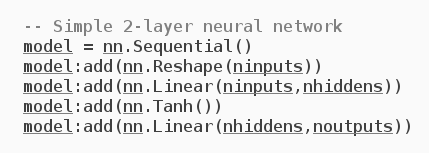
\includegraphics[width=8cm]{slike/nn_model.png}
\end{figure}

\end{frame}

\begin{frame}{Sustav za testiranje}

\begin{itemize}
\setlength\itemsep{0.5em}

	\item  Implementiran u jeziku C++ korištenjem OpenCV biblioteke
	
	\item Za pokretanje Torch modela koristi se C++ biblioteka JTorch
	
	\item Analiza točnosti klasifikacije 
	\begin{itemize}
		\item Matrica greške klasifikacije
 		\item Prikaz krivo klasificiranih primjera
	\end{itemize}
	
	\item Analiza kompleknosti modela
	\begin{itemize}
		\item Broj slobodnih parametara
 		\item Prosječno trajanje klasifikacije
	\end{itemize}
	
	\item Simultano analiziranje više modela
	\begin{itemize}
		\item Tablice točnosti po klasama
 		\item Tablice trajanja klasifikacije
	\end{itemize}
	
	
	
\end{itemize}


\end{frame}

\section{Rezultati}

\begin{frame}{Rezultati}

\begin{itemize}
\setlength\itemsep{0.5em}

 \item Modeli učeni i testirani na internim skupovima podataka tvrtke Microblink
 
 \item Slike znakova sa osobnih iskaznica, tzv. strojno čitljivih područja (MRZ)
 \begin{itemize}
 	\item  37 klasa znakova fonta ocrb
 	\item Obuhvaćaju znamenke, velika slova i znak manje
 \end{itemize}
 
 \item Sintetizirani skup podataka
 \begin{itemize}
 	\item  Dobiven slikanjem printanih imitacija osobnih iskaznica
 	\item  Više različitih modela mobitela i uvjeta osvijetljenja
 	\item 300 tisuća slika za učenje, 150 tisuća za testiranje
 \end{itemize}
 
 \item Ručno označeni skup podataka
 \begin{itemize}
 	\item  Dobiven slikanjem osobnih iskaznica u različitim uvjetima
 	\item  12 tisuća ručno označenih slika za testiranje
 \end{itemize}
 
\end{itemize}

\end{frame}


\begin{frame}{Rezultati}

\begin{itemize}
\setlength\itemsep{0.5em}

 \item Utjecaj predprocesiranja podataka
 
 \item Pronalaženje optimalne arhitekture
 \begin{itemize}
 	\item  Standarnih neuronskih mreža
 	\item Konvolucijskih neuronskih mreža
 \end{itemize}

 \item Usporedba optimalnih arhitektura
 \begin{itemize}
 	\item  Točnost klasifikacije
 	\item Kompleksnost i trajanje klasifikacije
 \end{itemize}
 
 \item Usporedba sa Microblink klasifikatorom
 
\end{itemize}

\end{frame}

\begin{frame}{Utjecaj predprocesiranja podataka}

\begin{figure}
\centering
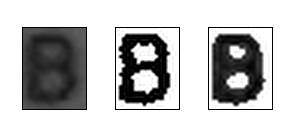
\includegraphics[width=10cm]{slike/preprocessing_comparison.png}
\end{figure}

\begin{table}
\begin{center}
\centering
\resizebox{\columnwidth}{!}{
    \begin{tabular}{ | c| c| c|c |}
    \hline
    Skup podataka & Adaptivni prag & Microblink interni & Bez predprocesiranja \\ \hline
    Sintetizirani & 98.29\% & 97.87\%  & 99.57\% \\ \hline
    Ručno označeni & 96.35\% & 97.66\% & 99.21\% \\  
    \hline
    \end{tabular}
}
\end{center}
\end{table}

\end{frame}

\begin{frame}{Pronalaženje optimalne standarne arhitekture}

\begin{figure}
\begin{center}
    \resizebox{.9\linewidth}{!}{% GNUPLOT: LaTeX picture with Postscript
\begingroup
  \makeatletter
  \providecommand\color[2][]{%
    \GenericError{(gnuplot) \space\space\space\@spaces}{%
      Package color not loaded in conjunction with
      terminal option `colourtext'%
    }{See the gnuplot documentation for explanation.%
    }{Either use 'blacktext' in gnuplot or load the package
      color.sty in LaTeX.}%
    \renewcommand\color[2][]{}%
  }%
  \providecommand\includegraphics[2][]{%
    \GenericError{(gnuplot) \space\space\space\@spaces}{%
      Package graphicx or graphics not loaded%
    }{See the gnuplot documentation for explanation.%
    }{The gnuplot epslatex terminal needs graphicx.sty or graphics.sty.}%
    \renewcommand\includegraphics[2][]{}%
  }%
  \providecommand\rotatebox[2]{#2}%
  \@ifundefined{ifGPcolor}{%
    \newif\ifGPcolor
    \GPcolorfalse
  }{}%
  \@ifundefined{ifGPblacktext}{%
    \newif\ifGPblacktext
    \GPblacktexttrue
  }{}%
  % define a \g@addto@macro without @ in the name:
  \let\gplgaddtomacro\g@addto@macro
  % define empty templates for all commands taking text:
  \gdef\gplbacktext{}%
  \gdef\gplfronttext{}%
  \makeatother
  \ifGPblacktext
    % no textcolor at all
    \def\colorrgb#1{}%
    \def\colorgray#1{}%
  \else
    % gray or color?
    \ifGPcolor
      \def\colorrgb#1{\color[rgb]{#1}}%
      \def\colorgray#1{\color[gray]{#1}}%
      \expandafter\def\csname LTw\endcsname{\color{white}}%
      \expandafter\def\csname LTb\endcsname{\color{black}}%
      \expandafter\def\csname LTa\endcsname{\color{black}}%
      \expandafter\def\csname LT0\endcsname{\color[rgb]{1,0,0}}%
      \expandafter\def\csname LT1\endcsname{\color[rgb]{0,1,0}}%
      \expandafter\def\csname LT2\endcsname{\color[rgb]{0,0,1}}%
      \expandafter\def\csname LT3\endcsname{\color[rgb]{1,0,1}}%
      \expandafter\def\csname LT4\endcsname{\color[rgb]{0,1,1}}%
      \expandafter\def\csname LT5\endcsname{\color[rgb]{1,1,0}}%
      \expandafter\def\csname LT6\endcsname{\color[rgb]{0,0,0}}%
      \expandafter\def\csname LT7\endcsname{\color[rgb]{1,0.3,0}}%
      \expandafter\def\csname LT8\endcsname{\color[rgb]{0.5,0.5,0.5}}%
    \else
      % gray
      \def\colorrgb#1{\color{black}}%
      \def\colorgray#1{\color[gray]{#1}}%
      \expandafter\def\csname LTw\endcsname{\color{white}}%
      \expandafter\def\csname LTb\endcsname{\color{black}}%
      \expandafter\def\csname LTa\endcsname{\color{black}}%
      \expandafter\def\csname LT0\endcsname{\color{black}}%
      \expandafter\def\csname LT1\endcsname{\color{black}}%
      \expandafter\def\csname LT2\endcsname{\color{black}}%
      \expandafter\def\csname LT3\endcsname{\color{black}}%
      \expandafter\def\csname LT4\endcsname{\color{black}}%
      \expandafter\def\csname LT5\endcsname{\color{black}}%
      \expandafter\def\csname LT6\endcsname{\color{black}}%
      \expandafter\def\csname LT7\endcsname{\color{black}}%
      \expandafter\def\csname LT8\endcsname{\color{black}}%
    \fi
  \fi
    \setlength{\unitlength}{0.0500bp}%
    \ifx\gptboxheight\undefined%
      \newlength{\gptboxheight}%
      \newlength{\gptboxwidth}%
      \newsavebox{\gptboxtext}%
    \fi%
    \setlength{\fboxrule}{0.5pt}%
    \setlength{\fboxsep}{1pt}%
\begin{picture}(7200.00,5040.00)%
    \gplgaddtomacro\gplbacktext{%
      \colorrgb{0.50,0.50,0.50}%
      \put(814,704){\makebox(0,0)[r]{\strut{}$92$}}%
      \colorrgb{0.50,0.50,0.50}%
      \put(814,1213){\makebox(0,0)[r]{\strut{}$93$}}%
      \colorrgb{0.50,0.50,0.50}%
      \put(814,1722){\makebox(0,0)[r]{\strut{}$94$}}%
      \colorrgb{0.50,0.50,0.50}%
      \put(814,2231){\makebox(0,0)[r]{\strut{}$95$}}%
      \colorrgb{0.50,0.50,0.50}%
      \put(814,2740){\makebox(0,0)[r]{\strut{}$96$}}%
      \colorrgb{0.50,0.50,0.50}%
      \put(814,3248){\makebox(0,0)[r]{\strut{}$97$}}%
      \colorrgb{0.50,0.50,0.50}%
      \put(814,3757){\makebox(0,0)[r]{\strut{}$98$}}%
      \colorrgb{0.50,0.50,0.50}%
      \put(814,4266){\makebox(0,0)[r]{\strut{}$99$}}%
      \colorrgb{0.50,0.50,0.50}%
      \put(814,4775){\makebox(0,0)[r]{\strut{}$100$}}%
      \colorrgb{0.50,0.50,0.50}%
      \put(1922,484){\makebox(0,0){\strut{}2}}%
      \colorrgb{0.50,0.50,0.50}%
      \put(2898,484){\makebox(0,0){\strut{}3}}%
      \colorrgb{0.50,0.50,0.50}%
      \put(3875,484){\makebox(0,0){\strut{}4}}%
      \colorrgb{0.50,0.50,0.50}%
      \put(4851,484){\makebox(0,0){\strut{}5}}%
      \colorrgb{0.50,0.50,0.50}%
      \put(5827,484){\makebox(0,0){\strut{}6}}%
      \colorrgb{0.50,0.50,0.50}%
      \put(6803,484){\makebox(0,0){\strut{}}}%
    }%
    \gplgaddtomacro\gplfronttext{%
      \csname LTb\endcsname%
      \put(176,2739){\rotatebox{-270}{\makebox(0,0){\strut{}Točnost klasifikacije (\%)}}}%
      \put(3874,154){\makebox(0,0){\strut{}Broj slojeva mreže}}%
      \csname LTb\endcsname%
      \put(5816,1097){\makebox(0,0)[r]{\strut{}Synth450}}%
      \csname LTb\endcsname%
      \put(5816,877){\makebox(0,0)[r]{\strut{}Manual}}%
    }%
    \gplbacktext
    \put(0,0){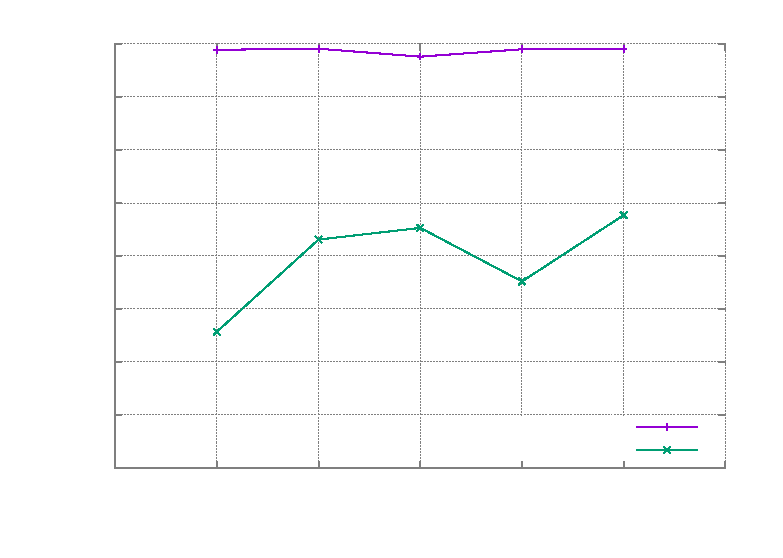
\includegraphics{grafovi/nn_complexity}}%
    \gplfronttext
  \end{picture}%
\endgroup
}
\end{center}
\end{figure}

\end{frame}

\begin{frame}{Pronalaženje optimalne konvolucijske arhitekture}

\begin{figure}
\begin{center}
    \resizebox{.9\linewidth}{!}{% GNUPLOT: LaTeX picture with Postscript
\begingroup
  \makeatletter
  \providecommand\color[2][]{%
    \GenericError{(gnuplot) \space\space\space\@spaces}{%
      Package color not loaded in conjunction with
      terminal option `colourtext'%
    }{See the gnuplot documentation for explanation.%
    }{Either use 'blacktext' in gnuplot or load the package
      color.sty in LaTeX.}%
    \renewcommand\color[2][]{}%
  }%
  \providecommand\includegraphics[2][]{%
    \GenericError{(gnuplot) \space\space\space\@spaces}{%
      Package graphicx or graphics not loaded%
    }{See the gnuplot documentation for explanation.%
    }{The gnuplot epslatex terminal needs graphicx.sty or graphics.sty.}%
    \renewcommand\includegraphics[2][]{}%
  }%
  \providecommand\rotatebox[2]{#2}%
  \@ifundefined{ifGPcolor}{%
    \newif\ifGPcolor
    \GPcolorfalse
  }{}%
  \@ifundefined{ifGPblacktext}{%
    \newif\ifGPblacktext
    \GPblacktexttrue
  }{}%
  % define a \g@addto@macro without @ in the name:
  \let\gplgaddtomacro\g@addto@macro
  % define empty templates for all commands taking text:
  \gdef\gplbacktext{}%
  \gdef\gplfronttext{}%
  \makeatother
  \ifGPblacktext
    % no textcolor at all
    \def\colorrgb#1{}%
    \def\colorgray#1{}%
  \else
    % gray or color?
    \ifGPcolor
      \def\colorrgb#1{\color[rgb]{#1}}%
      \def\colorgray#1{\color[gray]{#1}}%
      \expandafter\def\csname LTw\endcsname{\color{white}}%
      \expandafter\def\csname LTb\endcsname{\color{black}}%
      \expandafter\def\csname LTa\endcsname{\color{black}}%
      \expandafter\def\csname LT0\endcsname{\color[rgb]{1,0,0}}%
      \expandafter\def\csname LT1\endcsname{\color[rgb]{0,1,0}}%
      \expandafter\def\csname LT2\endcsname{\color[rgb]{0,0,1}}%
      \expandafter\def\csname LT3\endcsname{\color[rgb]{1,0,1}}%
      \expandafter\def\csname LT4\endcsname{\color[rgb]{0,1,1}}%
      \expandafter\def\csname LT5\endcsname{\color[rgb]{1,1,0}}%
      \expandafter\def\csname LT6\endcsname{\color[rgb]{0,0,0}}%
      \expandafter\def\csname LT7\endcsname{\color[rgb]{1,0.3,0}}%
      \expandafter\def\csname LT8\endcsname{\color[rgb]{0.5,0.5,0.5}}%
    \else
      % gray
      \def\colorrgb#1{\color{black}}%
      \def\colorgray#1{\color[gray]{#1}}%
      \expandafter\def\csname LTw\endcsname{\color{white}}%
      \expandafter\def\csname LTb\endcsname{\color{black}}%
      \expandafter\def\csname LTa\endcsname{\color{black}}%
      \expandafter\def\csname LT0\endcsname{\color{black}}%
      \expandafter\def\csname LT1\endcsname{\color{black}}%
      \expandafter\def\csname LT2\endcsname{\color{black}}%
      \expandafter\def\csname LT3\endcsname{\color{black}}%
      \expandafter\def\csname LT4\endcsname{\color{black}}%
      \expandafter\def\csname LT5\endcsname{\color{black}}%
      \expandafter\def\csname LT6\endcsname{\color{black}}%
      \expandafter\def\csname LT7\endcsname{\color{black}}%
      \expandafter\def\csname LT8\endcsname{\color{black}}%
    \fi
  \fi
    \setlength{\unitlength}{0.0500bp}%
    \ifx\gptboxheight\undefined%
      \newlength{\gptboxheight}%
      \newlength{\gptboxwidth}%
      \newsavebox{\gptboxtext}%
    \fi%
    \setlength{\fboxrule}{0.5pt}%
    \setlength{\fboxsep}{1pt}%
\begin{picture}(7200.00,5040.00)%
    \gplgaddtomacro\gplbacktext{%
      \colorrgb{0.50,0.50,0.50}%
      \put(814,704){\makebox(0,0)[r]{\strut{}$92$}}%
      \colorrgb{0.50,0.50,0.50}%
      \put(814,1213){\makebox(0,0)[r]{\strut{}$93$}}%
      \colorrgb{0.50,0.50,0.50}%
      \put(814,1722){\makebox(0,0)[r]{\strut{}$94$}}%
      \colorrgb{0.50,0.50,0.50}%
      \put(814,2231){\makebox(0,0)[r]{\strut{}$95$}}%
      \colorrgb{0.50,0.50,0.50}%
      \put(814,2740){\makebox(0,0)[r]{\strut{}$96$}}%
      \colorrgb{0.50,0.50,0.50}%
      \put(814,3248){\makebox(0,0)[r]{\strut{}$97$}}%
      \colorrgb{0.50,0.50,0.50}%
      \put(814,3757){\makebox(0,0)[r]{\strut{}$98$}}%
      \colorrgb{0.50,0.50,0.50}%
      \put(814,4266){\makebox(0,0)[r]{\strut{}$99$}}%
      \colorrgb{0.50,0.50,0.50}%
      \put(814,4775){\makebox(0,0)[r]{\strut{}$100$}}%
      \colorrgb{0.50,0.50,0.50}%
      \put(1678,484){\makebox(0,0){\strut{}5-10}}%
      \colorrgb{0.50,0.50,0.50}%
      \put(2410,484){\makebox(0,0){\strut{}8-15}}%
      \colorrgb{0.50,0.50,0.50}%
      \put(3142,484){\makebox(0,0){\strut{}10-20}}%
      \colorrgb{0.50,0.50,0.50}%
      \put(3875,484){\makebox(0,0){\strut{}13-25}}%
      \colorrgb{0.50,0.50,0.50}%
      \put(4607,484){\makebox(0,0){\strut{}15-30}}%
      \colorrgb{0.50,0.50,0.50}%
      \put(5339,484){\makebox(0,0){\strut{}18-35}}%
      \colorrgb{0.50,0.50,0.50}%
      \put(6071,484){\makebox(0,0){\strut{}20-40}}%
      \colorrgb{0.50,0.50,0.50}%
      \put(6803,484){\makebox(0,0){\strut{}}}%
    }%
    \gplgaddtomacro\gplfronttext{%
      \csname LTb\endcsname%
      \put(176,2739){\rotatebox{-270}{\makebox(0,0){\strut{}Točnost klasifikacije (\%)}}}%
      \put(3874,154){\makebox(0,0){\strut{}Broj mapa značajki u prvom i drugom sloju}}%
      \csname LTb\endcsname%
      \put(5816,1097){\makebox(0,0)[r]{\strut{}Synth450}}%
      \csname LTb\endcsname%
      \put(5816,877){\makebox(0,0)[r]{\strut{}Manual}}%
    }%
    \gplbacktext
    \put(0,0){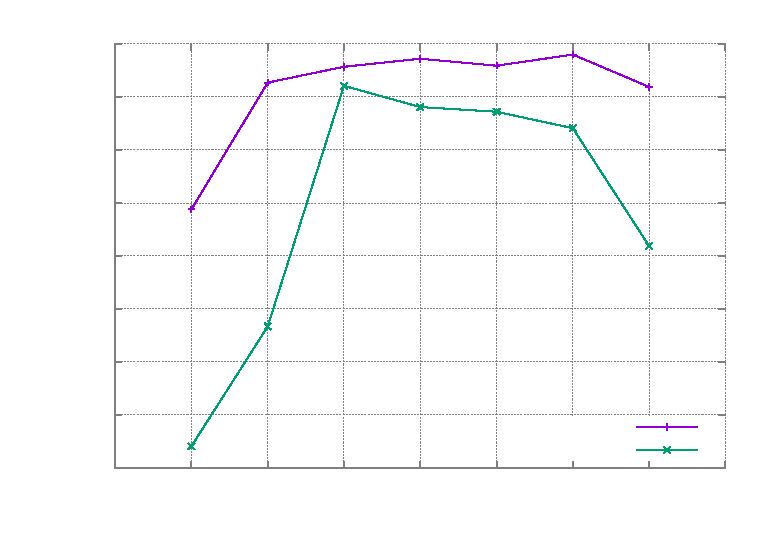
\includegraphics{grafovi/cnn_complexity}}%
    \gplfronttext
  \end{picture}%
\endgroup
}
\end{center}
\end{figure}

\end{frame}

\begin{frame}{Usporedba točnosti optimalnih arhitektura}
	
\begin{table}
\begin{center}
\centering
\resizebox{\columnwidth}{!}{
    \begin{tabular}{ | c| c| c|c |}
    \hline    		
    Skup podataka & Standarna arhitektura & Konvolucijska arhitektura \\ \hline
    Sintetizirani & 99.91\% & 99.57\%  \\ \hline
    Ručno označeni & 96.31\% & 	99.21\%  \\
    \hline
    \end{tabular}
}
\end{center}
\end{table}

\begin{itemize}
\setlength\itemsep{0.5em}
	\item  Konvolucijska arhitektura bolje generalizira na ručno označenom skupu
\end{itemize}

\begin{table}
\begin{center}
\centering
\resizebox{\columnwidth}{!}{
    \begin{tabular}{ | c| c| c|c | c| c| c|}
    \hline    		
    Arhitektura & Znamenka '0' & Slovo 'O' & Znamenka '8' & Slovo 'B'  \\ \hline
    Standarna & 74.15\% & 91.97\% & 98.69\% & 38.57\%  \\ \hline
    Konvolucijska & 97.55\% & 95.35\% & 99.81\% & 99.29\%   \\
    \hline
    \end{tabular}
}
\end{center}
\end{table}

\begin{itemize}
\setlength\itemsep{0.5em}
	\item Najveća razlika u točnosti kod teških slučajeva sličnih klasa 
\end{itemize}

\end{frame}

\begin{frame}{Usporedba kompleknosti optimalnih arhitektura}


\begin{table}
\begin{center}
\centering
\resizebox{\columnwidth}{!}{
    \begin{tabular}{ | c| c| c|c | c| c| c|}
    \hline    		
    Svojstvo & Standarna arhitektura & Konvolucijska arhitektura \\ \hline
    Računske operacije & 170550 & 97780  \\ \hline
    Slobodni parametri & 170550 & 6930   \\ \hline
    Trajanje klasifikacije  & 0.202 ms & 0.223 ms \\
    \hline
    \end{tabular}
}
\end{center}
\end{table}

\begin{itemize}
\setlength\itemsep{0.5em}

	\item  Po broju računskih operacija standarni model gotovo dvostruko kompleksniji, no prosječno trajanje klasifikacije je približno jednako
	
	\item Konvolucijska arhitektura ima za red veličine manji broj slobodnih parametara od standarne arhitekture
	
\end{itemize}


\end{frame}

\begin{frame}{Usporedba sa Microblink klasifikatorom}

\begin{table}
\begin{center}
\centering
    \begin{tabular}{ | c| c| c|c |}
    \hline    		
    Klasifikator & Sintetizirani skup  & Ručno označeni skup \\ \hline
    Microblink  & 86.93\% & 91.69\%  \\ \hline
    Standarna mreža & 99.91\% & 96.31\%  \\ \hline
    Konvolucijska mreža & 99.57\% &  99.21\% \\
    \hline
    \end{tabular}
\end{center}
\end{table}

\begin{itemize}
\setlength\itemsep{0.5em}
	\item Neuronske mreže bolje klasificiraju na oba testna skupa
\end{itemize}

\begin{table}
\begin{center}
\centering
    \begin{tabular}{ | c| c| c|c |}
    \hline    		
    Klasifikator & Prosječno trajanje klasifikacije \\ \hline
    Microblink & 0.025 ms \\ \hline
    Standarna mreža & 0.202 ms  \\ \hline
    Konvolucijska mreža &  0.223 ms \\
    \hline
    \end{tabular} 
\end{center}
\end{table}

\begin{itemize}
\setlength\itemsep{0.5em}
	\item Microblink klasifikator za red veličine brži od neuronskih mreža
\end{itemize}

\end{frame}

\begin{frame}{Zaključak}

\begin{itemize}
\setlength\itemsep{0.5em}

	\item  Pokazana je prednost prosljeđivanja neobrađenih slika dubokom klasifikatoru u svrhu očuvanja informacija slike 
	
	\item  Dodavanjem dubine bilo kojoj arhitekturi neuronske mreže pospješuje se njena sposobnost generalizacije
	
	\item Pokazana je prednost korištenja konvolucijske arhitekture zbog dodatnog ograničenja na njenu kompleksnost što pospješuje generalizaciju


	\item Rezultati klasifikatora tvrtke Microblink lošiji su od rezultata standarnih i konvolucijskih neuronskih mreža, što se može objasniti:
	 \begin{itemize}
 		\item  Negativnim utjecajem predprocesiranja podataka
 		\item Korištenjem značajki samo jedne razine apstrakcije
 \end{itemize}

	\item Naučene mreže su za red veličine sporije od Microblink klasifikatora, no još uvijek dovoljno brze za primjenu u stvarnom vremenu na mobilnom uređaju
	
\end{itemize} 
 
\end{frame}

\begin{frame}

\begin{center}
\large
 Hvala na pažnji!
\end{center}

\end{frame}

\end{document}